\documentclass{article}
\usepackage{amssymb}
\usepackage{tikz}
\usetikzlibrary{arrows,automata}
\newcounter{problem}
\newcounter{solution}

\newcommand\Problem{%
  \stepcounter{problem}%
  \textbf{\theproblem.}~%
  \setcounter{solution}{0}%
}

\newcommand\TheSolution{%
  \textbf{Solution:}\\%
}

\newcommand\ASolution{%
  \stepcounter{solution}%
  \textbf{Solution \thesolution:}\\%
}
\parindent 0in
\parskip 1em
\begin{document}

\begin{center}
\fbox{\fbox{\parbox{4in}{\centering Assignment 2 by Lucas Karlsson}}}
\end{center}

\Problem Give an informal, intuitive description of the language accepted by the DFA defined in the assignment question.

\TheSolution Below follows the automata you can design from the given DFA. Using this you can informally and intuitively describe what is going on. 

\begin{center}
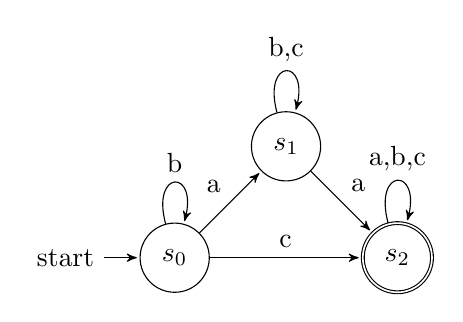
\begin{tikzpicture}[>=stealth',shorten >=1pt,auto,node distance=2cm]
  \node[state]         (s1)  {$s_1$};
  \node[initial,state] (s0) [below left of=s1]    {$s_0$};
  \node[state,accepting] (s2) [below right of=s1] {$s_2$};

  \path[->] (s0)  edge [loop above] node {b} (s0)
             edge              node {a} (s1)
             edge              node {c} (s2)
        (s1) edge [loop above] node {b,c} (s1)
             edge              node {a} (s2)
        (s2) edge [loop above] node {a,b,c} (s2);
        
\end{tikzpicture}
\end{center}

Basically, you can describe the language as following, every word has to either
tart by one or more b's or one c, if you start on one or more b's one a is 
directly followed then you can have zero or more b's or c's followed by another
a and then in the end you can have zero or more a's b's or c's. If you started 
with a c it will be followed by zero or more a's b's or c's. We could write it more 
formally as a regular expression "$b^*a(b+c)^*a(a+b+c)^* + b^*c(a+b+c)^*$"

Example of a word that would be accpeted by this language would be "bbabca" or just 
plain "c".

\newpage
\Problem In this exercise the alphabet $\Sigma = \{a,b\}$

\ASolution Here we want to define a DFA A over $\Sigma$ such that $L(A) = \{w \in \Sigma^* \mid \nexists u,v \in \Sigma^*. w = ubbav \}$. The solution for this is in the file "2point1ass2.jff". I'll explain what my automata does below.

\begin{center}
    "The words that is accepted by our language can start with 
    either one b or zero or more a's if we start with a b it 
    has to be followed by another a or one or more b and then 
    followed by an a into a unaccepted state that you cannot 
    escape. This translates into as soon as we get two or more 
    b's we will get stuck."
\end{center}

\ASolution Here we want to define a DFA B over $\Sigma$ that 
accepts exactly those string that have an even number of 
occurrences of a. The solution for this is in the file 
"2point2ass2.jff" I'll explain what my automata does below.

\begin{center}
    "The words that is accepted by our language can start with 
    either zero or more b's or one a followed by zero or more 
    b's followed by another a and we are back where we started.
    This way we only allow a even number of a's before we reach
    our final state." 
\end{center}
\newpage
\ASolution Here we want to construct $A \cdot B$ i.e use the product construction to 
build an automaton that accepts the language $L(A) \cap L(B)$. The solution for this 
is in the file "2point3ass2.jff" I wont explain what the automata does here because 
it heavily relies on my previous answers but i can explain the process of combining 
the two DFAs. To combine two DFAs we calculate $A \cdot B$ by doing 
$\{A_0,A_1,A_2,A_3\} \cdot \{B_0,B_1\}$ the new states will be:
\begin{center}
    $\{A_0B_0,A_0B_1,A_1B_0,A_1B_1,A_2B_0,A_2B_1,A_3B_0,A_3B_1\}$
\end{center}

To calculate the states and their transition functions we use the new states 
above and combine what a does to $A_0$ and $B_0$ and same for b and then the 
next state in the set. Below is the table that you can create by doing the 
method above.

\begin{table}[h!]
\centering
 \begin{tabular}{||c c c c||} 
 \hline
 & State & a & b \\ [0.5ex] 
 \hline\hline
 $\rightarrow$ $*$ (q0) & $A_0B_0$ & $A_0B_1$ & $A_1B_0$ \\ 
    \hfill          (q1) & $A_0B_1$ & $A_0B_0$ & $A_1B_1$ \\
    \hfill $*$ (q2) & $A_1B_0$ & $A_0B_1$ & $A_2B_0$ \\
    \hfill           (q3) & $A_1B_1$ & $A_0B_0$ & $A_2B_1$\\
    \hfill $*$ (q4) & $A_2B_0$ & $A_3B_1$ & $A_2B_0$ \\
    \hfill           (q5) & $A_2B_1$ & $A_3B_0$ & $A_2B_1$ \\
    \hfill           (q6) & $A_3B_0$ & $A_3B_1$ & $A_3B_0$ \\
    \hfill           (q7) & $A_3B_1$ & $A_3B_0$ & $A_3B_1$ \\[1ex] 
 \hline
 \end{tabular}
\end{table}
\begin{center}
  We can then use this table to construct our automata using JFLAP, which is what we have done in the file mentioned above and it will hold for $L(A) \cap L(B)$.
\end{center} 
\newpage
\Problem In this exercise the alphabet $\Sigma = \{a,b\}$

\ASolution We want to define a NFA A without 
$\epsilon$-transitions over $\Sigma$ such that $L(A) = M \cup 
N$ where $M=\{w \in \Sigma^* \mid \exists u,v \in \Sigma^*. w =
ubaav\}$ And N contains exactly those strings in $\Sigma^*$ 
where every occurence of a is directly followed by two or more 
occurences of b.

Defining M, we want M to only contain words that contain the substring "baa". 
We can do this using the following automata:

\begin{center}
\begin{tikzpicture}[>=stealth',shorten >=1pt,auto,node distance=2cm]
  \node[initial,state, accepting] (s0) [left of=s1]    {$m_0$};
  \node[state] (s1)  {$m_1$};
  \node[state] (s2) [above right of=s1]  {$m_2$};
  \node[state, accepting] (s3) [below right of=s2] {$m_3$};

  \path[->] (s0)  edge [loop above] node {b} (s0)
             edge              node {a} (s1)
        (s1) edge              node {b} (s2)
        (s2) edge              node {b} (s3)
        (s3) edge [loop above] node {b} (s3)
             edge              node {a} (s1);
        
\end{tikzpicture}
\end{center}

Defining N, we want N where every time we have a occurence of a is followed by two occurences of b. We can do this using the following automata:

\begin{center}
\begin{tikzpicture}[>=stealth',shorten >=1pt,auto,node distance=2cm]
  \node[initial,state] (s0) [left of=s1]    {$n_0$};
  \node[state] (s1)  {$n_1$};
  \node[state] (s2) [right of=s1]  {$n_2$};
  \node[state, accepting] (s3) [right of=s2] {$n_3$};

  \path[->] (s0)  edge [loop above] node {a,b} (s0)
                  edge              node {b} (s1)
        (s1) edge              node {a} (s2)
        (s2) edge              node {a} (s3)
        (s3) edge [loop above] node {a,b} (s3);
        
\end{tikzpicture}
\end{center}

Now we have to combine M and N by creating a new initial state that acts 
as both the M initial state and N initial state this can be done by adding
the $q_0$ state below 
\begin{center}
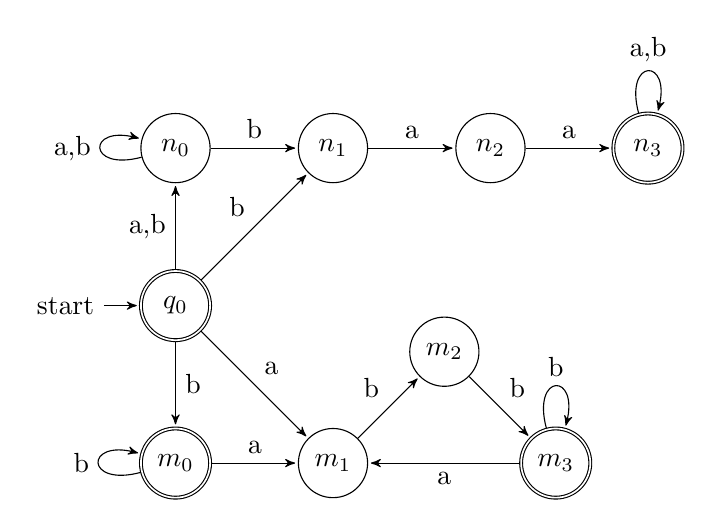
\begin{tikzpicture}[>=stealth',shorten >=1pt,auto,node distance=2cm]
  \node[state] (n0)   {$n_0$};
  \node[state] (n1) [right of=n0] {$n_1$};
  \node[state] (n2) [right of=n1]  {$n_2$};
  \node[state, accepting] (n3) [right of=n2] {$n_3$};
  
  \node[state, accepting, initial] (q0) [below of=n0] {$q_0$};
  
  \node[state, accepting] (m0) [below of=q0]    {$m_0$};
  \node[state] (m1) [right of=m0] {$m_1$};
  \node[state] (m2) [above right of=m1]  {$m_2$};
  \node[state, accepting] (m3) [below right of=m2] {$m_3$};

  \path[->] (n0)  edge [loop left] node {a,b} (n0)
                  edge             node {b} (n1)
        (n1) edge                  node {a} (n2)
        (n2) edge                  node {a} (n3)
        (n3) edge [loop above]     node {a,b} (n3);
        
  \path[->] (q0)  edge             node {b} (m0)
                  edge             node {a} (m1)
                  edge             node {b} (n1)
                  edge             node {a,b} (n0);

  \path[->] (m0)  edge [loop left] node {b} (m0)
             edge                  node {a} (m1)
        (m1) edge                  node {b} (m2)
        (m2) edge                  node {b} (m3)
        (m3) edge [loop above]     node {b} (m3)
             edge                  node {a} (m1);
    
        
\end{tikzpicture}
\end{center}
 
You can now use $q_0$ as the initial state both for M and N and such we 
have solved the problem. This is also the automata found in the file "3point1ass2.jff".
 
\ASolution We want to use the subset construction to build a 
corresponding DFA and we are allowed to omit inaccesible 
states.asd

\end{document}
